\documentclass[12pt]{article}
\usepackage{amsmath}
\usepackage[utf8]{inputenc}
\usepackage[russian]{babel}
\usepackage{color}
\usepackage[usenames,dvipsnames]{xcolor}
\usepackage{graphicx}

\title{Математический анализ. Контрольная работа №2 - Роман Гафиятуллин (192001-04)}
\author{Роман Гафиятуллин (БГУИР)}

\begin{document}
	\begin{titlepage}
		\begin{center}
			{\Large Математический анализ. \\ Контрольная работа №2 \\ Роман Гафиятуллин (192001-04)}
		\end{center}
	\end{titlepage}
	%%%%%%%%%%%%%%%%%%%%%%%%%%%%%%%%%%%%%%%%%%%%%%%%%%%%%%%%%%%%%%%%%%%%%%%%%%%%%%%%%%%%%%%%%%%%%%%%%%%%%%%%%%%%%%
	\clearpage
	\paragraph{04-2.1} 
		Найти производные \ensuremath{\frac{dy}{dx}} следующих функций. \\
	\begin{description}
		\item[а)]
			\ensuremath{
				y = ln( x + \sqrt{x^2 + 1} ) \\
				\textcolor{Cyan}{// f = ln \circ g(x)} \\
				\textcolor{Cyan}{// g = x^2 + 1} \\
				\textcolor{Cyan}{// y' = f' \circ g(x) \cdot g'(x) } \\
				y' = ln'( x^2 + 1 ) \cdot (x^2 + 1)' = \\
				= ( x^1 + 1 )^{-1} \cdot 2x + 0 = \\
				= {\bf \frac{2x}{ x^1 + 1 } }
			}
		\item[б)]
			\ensuremath{
				y = \frac
					{1 - cos(3x)}
					{1 + cos(3x)} \ | \ 3x \, mod \, 2\pi \neq \pi
				\\\\
				\textcolor{Cyan}{
					// u = 3x
				} \\
				y = \frac
						{1 - cos \, u}
						{1 + cos \, u} \\
				\textcolor{Cyan}{ // g(u) = 1 - cos \, u } \\
				\textcolor{Cyan}{ // h(u) = 1 + cos \, u } \\
				\textcolor{Cyan}{ // g'(u) = sin \, u} \\
				\textcolor{Cyan}{ // h'(u) = -sin \, u} \\
				\textcolor{Cyan}{ 
					// ( \frac{g(u)}{h(u)} )' 
					= \frac{ g'(u) \cdot h(u) - h'(u) \cdot g(u) }{ h(u)^2 }
				} \\
				\frac{d y}{d u} = 
					\frac
						{ sin \, u \cdot (1 + cos \, u) + sin \, u \cdot ( 1 - cos \, u ) }
						{ (1 + cos \, u)^2 } = \frac{ 2 sin \, u}{(cos \, u + 1)^2} \\
				\\
				\textcolor{Cyan}{ 
					// f(u) = \frac
								{ 1 - cos \, u }
								{ 1 + cos \, u }
				} \\
				\textcolor{Cyan}{
					// f'(u) = \frac{ 2 sin \, u}{(cos \, u + 1)^2}
				} \\
				\textcolor{Cyan}{ // u(x) = 3x } \\
				\textcolor{Cyan}{ // u'(x) = 3 } \\
				\textcolor{Cyan}{ // y = f \circ u (x) } \\
				\textcolor{Cyan}{ // y' = f' \circ u(x) \cdot u'(x) } \\
				y' = ( \frac{ 2 \cdot sin(3x) }{ (cos (3x) + 1 )^2} ) \cdot 3 = \\
				= 
				{\bf \frac
					{6 \cdot sin(3x)}
					{(cos(3x) + 1)^2}
				}
			}
		\item[в)]
			\ensuremath{
				x = t^4 + 2t,\, y = t^2 + 5t
				\\
				\textcolor{Cyan}{ 
					// \frac{dy}{dx} = \frac{d y}{d t} \cdot \frac{d t}{d x} 
						= \frac{ \frac{d y}{d t} }{ \frac{d x}{d t} }
				} \\
				\frac{d y}{d t} = 2t + 5 \\
				\frac{d x}{d t} = 4t + 2 \\
				{\bf \frac{d y}{d x} = \frac{2t + 5}{4t + 2} }
			}
	\end{description}
	%%%%%%%%%%%%%%%%%%%%%%%%%%%%%%%%%%%%%%%%%%%%%%%%%%%%%%%%%%%%%%%%%%%%%%%%%%%%%%%%%%%%%%%%%%%%%%%%%%%%%%%%%%%%%%
	\paragraph{04-2.2} 
		Найти пределы функции, применяя правило Лопиталя. \\
	\ensuremath{
		\lim_{x \to 1} 
			\frac
				{ 1 - x^2 }
				{ ln x } = \frac{0}{0} \textcolor{Cyan}{ \mbox{ // Можно применять правило Лопиталя } } \\
		\lim_{x \to 1}
			\frac
				{ 1 - x^2 }
				{ ln x } 
		= \lim_{x \to 1} \frac
							{ (1 - x^2)' }
							{ (ln x)' } = \\
		= \lim_{x \to 1}	\frac
							{ -2x }
							{ \frac{1}{x} }
		= \lim_{x \to 1} -2 x^2 = -2 ( \lim_{x \to 1} x )^2 = {\bf -2 }
	}

	%%%%%%%%%%%%%%%%%%%%%%%%%%%%%%%%%%%%%%%%%%%%%%%%%%%%%%%%%%%%%%%%%%%%%%%%%%%%%%%%%%%%%%%%%%%%%%%%%%%%%%%%%%%%%%
	\paragraph{04-2.3} 
		Методами дифференциального исчисления исследовать функцию \ensuremath{y = f(x)} и по результатам исследования построить ее график. 
		Найти наименьшее и наибольшее значения функции на отрезке \ensuremath{ [ \, a ; b \, ] }. \\
	\begin{description}
		\item[функция:]
			\ensuremath{
				y = \frac
					{ x ^2 - 5 }
					{ x - 3 }
			}
		\item[отрезок:]
			\ensuremath{
				[ \, -2; 2 \, ]
			}
	\end{description}

	%%%%%%%%%%%%%%%%%%%%%%%%%%%%%%%%%%%%%%%%%%%%%%%%%%%%%%%%%%%%%%%%%%%%%%%%%%%%%%%%%%%%%%%%%%%%%%%%%%%%%%%%%%%%%%
	\paragraph{04-2.4} 
		Задана функция \ensuremath{y = f(x)}. 
		Установить, является ли данная функция непрерывной.
		В случае разрыва функции в некоторой точке найти ее пределы слева и справа, классифицировать характер разрыва.
		Построить схематично график функции.

	\ensuremath{
		y = \left \{ \begin{array}{rl}
			cos x, &\mbox{ $x \le 0$ }; \\
			x ^2 + 1, &\mbox{ $0 < x < 1$ }; \\
			x, &\mbox{ $x \ge 1$ }.
		\end{array} \right .
	}
	\\\\
	\ensuremath{
		\left.\begin{array}{rl}
			cos x = 1, \, x = 0 \\
			\lim_{ x \to 0+ } \, x ^2 + 1 = 1 \\
		\end{array} \right \} \Rightarrow 
	} Функция неразрывна при \ensuremath{ x \in (-\infty; 1) }
	\\\\
	\ensuremath{
		\left.\begin{array}{rl}
			\lim_{ x \to 1- } \, x ^2 + 1 = 2 \\
			x = 1 \, \mbox{ при x = 1 }
		\end{array} \right \} \Rightarrow
		\vbox{
			Разрыв первого рода: функция определена в точке \ensuremath{x = 1}, \\
			односторонний предел слева существует и конечен.
		}
	}
	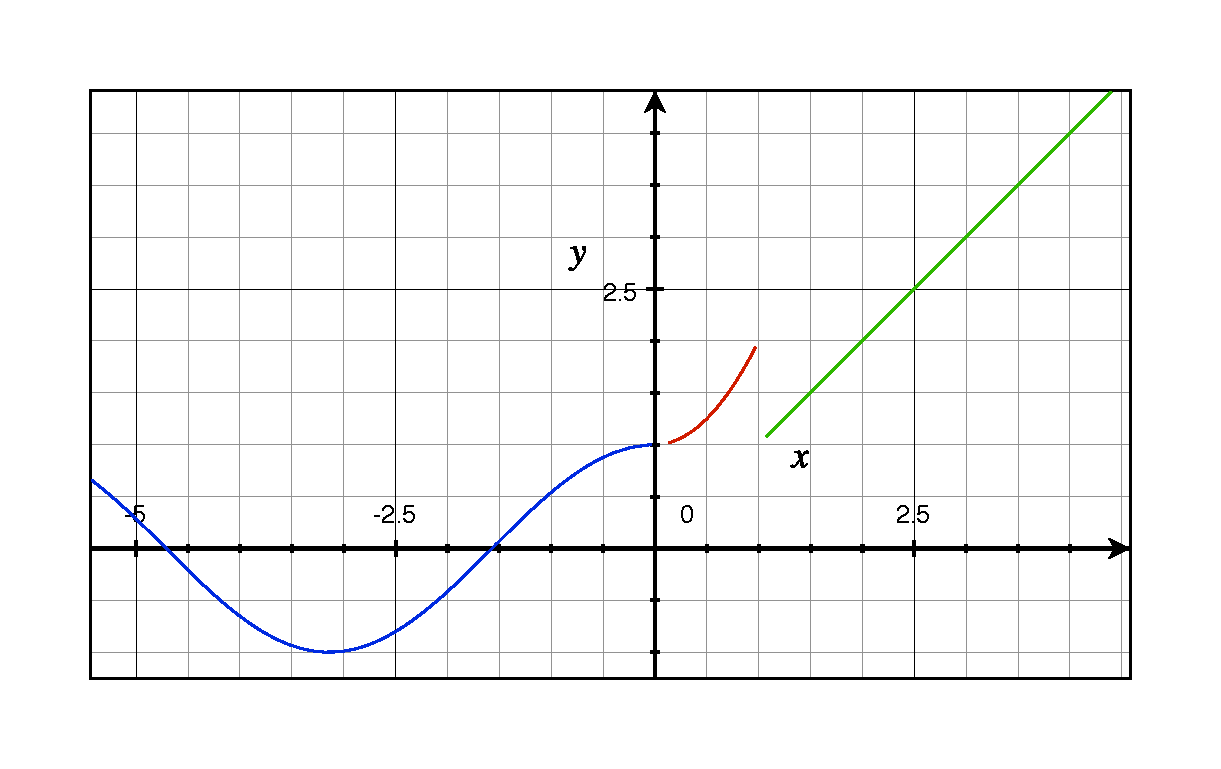
\includegraphics[width=450px,height=250px]{RG-Uni-Calculus-Reference_Work_1-04-1-5.eps}


\end{document}

